\documentclass[12pt]{exam}

%: ****Input files for all exams****
% (all input files require a file path that will change if the location of this document changes)

% The preamble provides all the instructions for how the whole document works, this includes which packages of code can be used. It generally does not need editing while making the exam.
\input{a2preamble}

%: ****Input files specific to course exam****

%These input files include booleans for turning on or off various versions as well as specific codes for a particular course. It can be helpful to have these open while writing the exam

% Boolean files are specific to the exam so that changing a true/false does not change all exams.
\input{a2boolean}
%\input{Algebra 1 Exam Boolean (Input File) SY26V1}
%\input{Algebra 2 Exam Boolean (Input File) SY26V1}
%\input{Geometry Exam Boolean (Input File) SY26V1}
%\input{Pre-Calculus Exam Boolean (Input File) SY26V1}

%Algebra Courses - Styles and Symbols
\input{a2tikz}
%Geometry Courses - Styles and Symbols
% \input{a2symbols}

%%%%%%%%%%%%%%%%%%%%%%%%%%%%%%%%%%%%%%%%%%%%%%%
%: Begin Document
%%%%%%%%%%%%%%%%%%%%%%%%%%%%%%%%%%%%%%%%%%%%%%%
\begin{document}
\thispagestyle{head} %Enacts header code

%%%%%%%%%%%%%%%%%%%%%%%%%%%%%%%%%%%%%%%%%%%%%%%
%: Coverpage
%%%%%%%%%%%%%%%%%%%%%%%%%%%%%%%%%%%%%%%%%%%%%%%
\begin{coverpages}
%: Exam Title
\examTitle{
 Algebra 2 
}{
Final Exam %Final or Midterm
}{
May 27, 2026 %Date
}

%: 	Directions
%\examDirections{Universal Directions}{Supported Directions}{Modified Directions}{MLL Directions){Extra Time Directions}
\examDirections{
    %Universal Directions
    You have \ifExtraTime{up to 3 hours}{2 hours} in which to complete this portion of the exam. All work must be your own. If at any point during this exam you are seen accessing a phone\ifStan{, notes, or any other material,}{ or computer } your test will be taken and you will not have the opportunity to continue.
    
        \ifESP{ %Spanish translation
        	\textcolor{blue!80!black}{Usted tiene 2 horas para completar esta porción del examen. Todo el trabajo debe ser de su propia autoría. Si en cualquier momento durante este examen se le ve utilizando un teléfono, notas, o cualquier otro material, se le retirará su examen y no tendrá la oportunidad de continuar.}
        }{} 
    
    \vspace{3mm}
    
    Mark all answers on the Answer Sheet. Do {\bf NOT} damage, fold, or doodle on the Answer Sheet. Mark your answers by darkly filling in the circle with a pencil. To change your answer, erase as completely as possible, and pick a new choice.
    
    \vspace{3mm}
    
    Please write down work on the blank spaces of this test packet. If you need more blank pages, please ask the proctor. At the end of the test, hand in {\bf all} pages.
    
    \vspace{3mm}
    
    You may use a scientific calculator throughout this exam. Before you hand in your exam, write your end time on the Support Documentation page (back of this page).
    
        \ifESP{ %Spanish translation
            \textcolor{blue!80!black}{Asegúrese de mostrar todo su trabajo y organizarlo de forma ordenada. Puede usar una calculadora científica durante todo el examen. Antes de entregar su examen, escriba su hora de finalización en la página de Documentación de Apoyo.}
        }{}

}{
    %Supported Directions
    This is a supported version of the exam. Problems may have additional steps to support your thinking process. An example or model problem may be given. Terms may be defined. 
    
        \ifESP{ %Spanish translation
            \textcolor{blue!80!black}{
            Esta es una versión del examen con apoyos. Los problemas pueden tener pasos adicionales para apoyar su proceso de pensamiento. Se puede proporcionar un ejemplo o un problema modelo. Los términos pueden estar definidos.
            }
        }{}
}{
    %Modified Directions
    This is a modified version of the exam. There are fewer questions, and some questions have been simplified.
    %Problems will have additional steps to support your thinking process and there may be shorter or fewer questions on the exam. Vocabulary is defined and symbol banks are provided.
}{
    %MLL Support Directions
    This exam has supports for Multi-Lingual Learners. Supports include: underlining key words, providing translations of key words, explanations in Spanish, and an English-Spanish glossary. 
    
    %Spanish translation
    \textcolor{blue!80!black}{Este examen cuenta con apoyos para Estudiantes Multilingües. Los apoyos incluyen: el subrayado de palabras clave, la provisión de traducciones de palabras clave, explicaciones en español y un glosario inglés-español.}
}{
    %Extra time Directions
    You have extra time on this exam. You have up to 3.5 hours. After 2 hours there will be a 10 minute break for all students. If you finish the exam before 3.5 hours, you may hand it in and get permission to leave the exam room. 
} %End \examDirections


%:	Pledge Box
\pledgeBox

\newpage

%: 	Accommodations and Modifications
%: 		Support Documentation Page
\SupportDocumentation{
%: 			General Classroom Accommodations
\begin{itemize}[itemsep=-4pt]
\item Check-in if attention wanders or student appears stuck.
\item Prompt student to read directions, read directions aloud to student.
\item If student turns in exam early, teacher reviews exam to ensure all problems are answered.
\item Provide time updates, remind students to look at all problems.
\item Access to a scientific calculator (not on the Chromebook).
\end{itemize}
}{
%:			Specific Accommodations and Modifications

\ifStan{
%:				ST
Standard Test:
\begin{checklist}[itemsep=3pt, parsep=-3pt]
% \item[\ifExtraSpace{\true}{\false}] Extra Space: additional space provided on writing problems and proofs.
\ifExtraTime{\item[\true]Extra time: Student has up to 1.5 additional hours unless otherwise noted.}{}
\item[\true] No additional accommodations or modifications
\end{checklist}
}{}

\ifMod{
%:				M
Modified Test: 
\begin{checklist}[itemsep=3pt, parsep=-3pt]
\ifModSup{
% \item[\ifExtraSpace{\true}{\false}] Extra Space: additional space provided on writing problems and proofs.
\item[\ifExtraTime{\true}{\false}]Extra time: Student has up to 1.5 additional hours unless otherwise noted.
\item[\true] Student can use practice final and notes.
\item[\true] Simplified questions
% \item[\true] Defined vocabulary
% \item[\true] Recall prompts provided
% \item[\true] Problems broken into steps
% \item[\true] Prompts to remember strategies we've used in class
% \item[\true] Graphic organizers to prompt specific strategies 
%\item[\true] Reduced options on multiple choice
}{}
\item[\true] Reduced number of questions
\end{checklist}
}{}
\ifSup{
%:				SP
Supported Test:
\begin{checklist}[itemsep=3pt, parsep=-3pt]
\item[\ifExtraSpace{\true}{\false}] Extra Space: additional space provided on writing problems and proofs.
\item[\ifExtraTime{\true}{\false}]Extra time: Student has up to 1.5 additional hours unless otherwise noted. 
\item[\true] Vocabulary Reference sheet
\item[\true] Recall prompts provided
\item[\true] Problems broken into steps
\item[\true] Graphic organizers to prompt specific strategies 
%\item[\true] Reduced options on multiple choice
\end{checklist}
}{}
\ifESP{
MLL Supports: 
\begin{checklist}[itemsep=3pt, parsep=-3pt]
\item[\true] English-Spanish Glossary Reference Sheet
\item[\true] Key words underlined
\item[\true] Explanations and Important words or directions translated
\end{checklist}
}{}
}{
%: 	Additional Supports
\textbf{Additional Support:}

\vspace{-2mm}
\begin{checklist}[itemsep=3pt, parsep=-3pt]
\item Redirected attention
\item Scribed for student
\item Encouraged student to write more/look at a problem again
\item Verbally walked student through directions
\item Restated directions in a different way
\item Defined vocabulary or gave an example of how a symbol would be used
\end{checklist}
}

% \newpage
% % \blankpage
% 
% This page is intentionally left blank.
% 
% \newpage
% % \blankpage
% 
% This page is intentionally left blank.
% 


\end{coverpages}

%%%%%%%%%%%%%%%%%%%%%%%%%%%%%%%%%%%%%%%%%%%%%%%
%: Reference Sheets
%%%%%%%%%%%%%%%%%%%%%%%%%%%%%%%%%%%%%%%%%%%%%%%


%%%%%%%%%%%%%%%%%%%%%%%%%%%%%%%%%%%%%%%%%%%%%%%
%: Questions
%%%%%%%%%%%%%%%%%%%%%%%%%%%%%%%%%%%%%%%%%%%%%%%
\begin{questions}

%: Solve two-step linear equation
\question Solve the linear equation.
$$5=\frac{x}{3}-2$$
\begin{choices} 
	\choice $x=13$
	\choice $x=17$
	\choice $x=19$
	\correctchoice $x=21$ 
\end{choices}

\vfill

%: Evaluate function
\question Let function $f$ be defined by the algebraic expression below:
$$f(x)=\frac{5-x}{2}$$
Evaluate $f(-3)$.
\begin{choices} 
	\choice $f(-3)=1$
	\choice $f(-3)=2$
	\correctchoice $f(-3)=4$
	\choice $f(-3)=8$ 
\end{choices}

\vfill


%: Inverse of cube-root function
\question Let function $f$ be defined by the algebraic expression below.
$$f(x)=\sqrt[3]{x+2}-5$$
Find the inverse of function $f$.
\begin{choices} 
	\correctchoice $f^{-1}(x)=(x+5)^3-2$
	\choice $f^{-1}(x)=(x+5)^3+2$
	\choice $f^{-1}(x)=(x+2)^3-5$
	\choice $f^{-1}(x)=(x+2)^3+5$
\end{choices}

\vfill

\newpage

%: Is relation a function?
\question Consider the relation shown by the curve below.

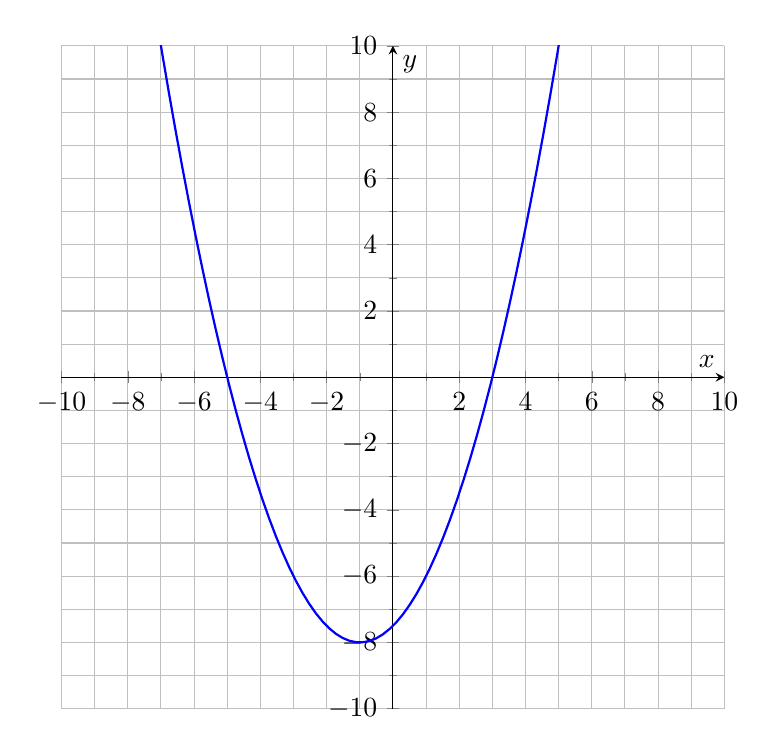
\begin{tikzpicture}
    \begin{axis}[
        axis lines = middle,
        xlabel = {$x$},
        ylabel = {$y$},
        xmin = -10, xmax = 10,
        ymin = -10, ymax = 10,
        grid = both,
        minor tick num = 1,
        width = 10cm,
        height = 10cm,
        legend pos = north west,
    ]
    
    % Plot f(x) = 1/2*(x+5)+4
    \addplot [
        domain=-10:10, 
        samples=100, 
        color=blue,
        thick,
    ]
    {0.5*(x+1)^2-8};
    
    \end{axis}
\end{tikzpicture}

\begin{choices} 
	\choice The relation represents a one-to-one function because it passes both the vertical line test and the horizontal line test.
	\correctchoice $y$ is a function of $x$ because the relation passes the vertical line test, but $x$ is {\bf NOT} a function of $y$ because the relation fails the horizontal line test.
	\choice $x$ is a function of $y$ because the relation passes the horizontal line test, but $y$ is {\bf NOT} a function of $x$ because the relation fails the vertical line test.
	\choice Neither $x$ nor $y$ is a function of the other because the relation fails both the vertical and horizontal line tests.
\end{choices}

\vfill

\ifStan{
%: Solve radical equation
\question Solve the radical equation.
$$8=17-\sqrt{3x}$$
\begin{choices} 
	\choice $x=3$
	\choice $x=9$
	\correctchoice $x=27$
	\choice $x=81$
\end{choices}

\vfill
}{
\question Solve the radical equation.
$$5\cdot \sqrt{x+2} = 15$$
\begin{choices} 
	\choice $x=5$
	\choice $x=6$
	\correctchoice $x=7$
	\choice $x=8$
\end{choices}

\vfill
}

\newpage

%: Get rational solutions to factored quadratic
\question Find the solutions to the factored quadratic equation.
$$(2x-3)(5x+7)=0$$
\begin{choices} 
	\correctchoice $x=\frac{3}{2}$ and $x=\frac{-7}{5}$
	\choice $x=\frac{-3}{2}$ and $x=\frac{7}{5}$
	\choice $x=\frac{2}{3}$ and $x=\frac{-5}{7}$
	\choice $x=\frac{-2}{3}$ and $x=\frac{5}{7}$
\end{choices}

\vfill

%: State quadratic formula
\question The quadratic formula states that if $ax^2+bx+c=0$, then:
\begin{choices} 
	\choice $x=\frac{b\pm\sqrt{b^2+4ac}}{2a}$
	\choice $x=\frac{-b\pm\sqrt{b^2+4ac}}{2a}$
	\choice $x=\frac{b\pm\sqrt{b^2-4ac}}{2a}$
	\correctchoice $x=\frac{-b\pm\sqrt{b^2-4ac}}{2a}$
\end{choices}

\vfill

%: Factor quadratic expression
\question Factor the quadratic expression. $$x^2+3x-4$$
\begin{choices} 
	\choice $(x+2)(x-2)$
	\correctchoice $(x+4)(x-1)$
	\choice $(x-2)(x-2)$
	\choice $(x-3)(x-1)$
\end{choices}

\vfill

\ifStan{
%: Factor quadratic expression with leading coefficient
\question Factor the quadratic expression $6x^2+x-12$.

\begin{choices} 
	\choice $(6x+1)(x-12)$
	\choice $(6x-1)(x+12)$
	\choice $(3x+4)(2x-3)$
	\correctchoice $(3x-4)(2x+3)$
\end{choices}

\vfill
}


\newpage

%: Expand quadratic expression
\question Expand the quadratic expression $(x+1)(x+2)$

\begin{choices} 
	\choice $x^2+2$
	\choice $2x+3$
	\correctchoice $x^2+3x+2$
	\choice $x^2+x+3$
\end{choices}

\vfill


\ifStan{
%: Rationalize denominator
\question Rationalize the denominator. Remember, $i=\sqrt{-1}$. $$\frac{1+2i}{4+3i}$$

\begin{choices} 
	\choice $\frac{3+8i}{7}$
	\choice $\frac{10+5i}{7}$
	\choice $\frac{11+2i}{25}$
	\correctchoice $\frac{2+i}{5}$
\end{choices}

\vfill
}

\ifStan{
%: Expand quadratic expression with complex roots
\question Expand the quadratic polynomial with complex roots $$(x-6-7i)(x-6+7i)$$

\begin{choices} 
	\choice $x^2-12x+13$
	\correctchoice $x^2-12x+85$
	\choice $x^2+12x+13$
	\choice $x^2+12x+85$
\end{choices}

\vfill
}{
\question Multiply the complex numbers. $$(5+2i)\cdot (3-4i)$$

\begin{choices} 
	\choice $7+2i$
	\correctchoice $23-14i$
	\choice $15-8i$
	\choice $-20+6i$
\end{choices}

\vfill
}

%: Find complex solutions of quadratic polynomial
\ifStan{
\question Find both solutions to the quadratic equation. (Each choice represents two possible solutions, so only choose one of the four choices.)
$$0=x^2-8x+28$$
}{
\question Use the quadratic formula to find both solutions to the quadratic equation. (Each choice represents two possible solutions, so only choose one of the four choices.)
$$0=x^2-8x+28$$
}


\begin{choices} 
	\correctchoice $x=4\pm 2i\sqrt{3}$
	\choice $x=4\pm 3i\sqrt{2}$
	\choice $x=4\pm4i\sqrt{11}$
	\choice $x=4\pm4i\sqrt{6}$
\end{choices}

\vfill

\newpage

The next 4 problems all refer to the diagram below.

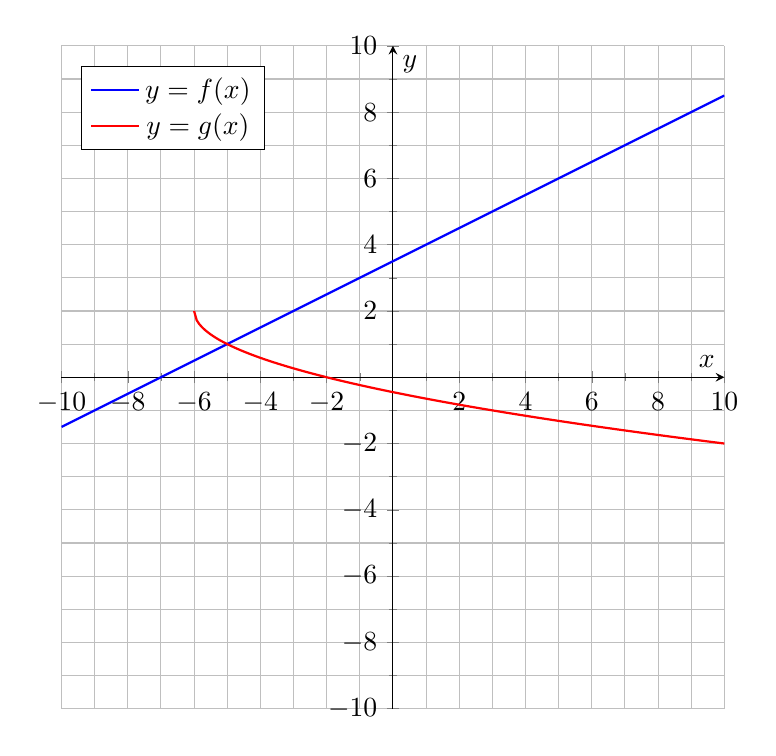
\begin{tikzpicture}
    \begin{axis}[
        axis lines = middle,
        xlabel = {$x$},
        ylabel = {$y$},
        xmin = -10, xmax = 10,
        ymin = -10, ymax = 10,
        grid = both,
        minor tick num = 1,
        width = 10cm,
        height = 10cm,
        legend pos = north west,
    ]
    
    % Plot f(x) = 1/2*(x+5)+4
    \addplot [
        domain=-10:10, 
        samples=100, 
        color=blue,
        thick,
    ]
    {0.5*(x+5)+1};
    \addlegendentry{$y=f(x)$}

    % Plot g(x) = -sqrt(x+6)+5
    % Note: domain starts at -6 because the square root is undefined for x < -6
    \addplot [
        domain=-6:10, 
        samples=200, 
        color=red,
        thick,
    ]
    {-sqrt(x+6)+2};
    \addlegendentry{$y=g(x)$}
    
    \end{axis}
\end{tikzpicture}


%: Find point-slope equation from graph
\question What is the equation of the line in point-slope form?

\begin{choices} 
	\choice $f(x)=\frac{1}{2}(x-5)+1$
	\correctchoice $f(x)=\frac{1}{2}(x+5)+1$
	\choice $f(x)=\frac{1}{2}(x-5)-1$
	\choice $f(x)=\frac{1}{2}(x+5)-1$
\end{choices}


%: Find radical equation from graph
\question What is the equation of the radical curve?

\begin{choices} 
	\correctchoice $g(x)=-\sqrt{x+6}+2$
	\choice $g(x)=\sqrt{-(x+6)}+2$
	\choice $g(x)=-\sqrt{x-6}+2$
	\choice $g(x)=\sqrt{-(x-6)}+2$
\end{choices}


%: Find actual solution of linear-radical system
\question What is the valid solution to $f(x)=g(x)$?

\begin{choices} 
	\choice $x=-6$
	\correctchoice $x=-5$
	\choice $x=3$
	\choice $x=4$
\end{choices}

%: Find extraneous solution of linear-radical system
\question What is the extraneous solution to $f(x)=g(x)$?

\begin{choices} 
	\choice $x=-6$
	\choice $x=-5$
	\correctchoice $x=3$
	\choice $x=4$
\end{choices}

\newpage


%: Power of i
\question Let $i=\sqrt{-1}$. Simplify $i^{67}$.

\begin{choices} 
	\choice $i$
	\choice $-1$
	\correctchoice $-i$
	\choice $1$
\end{choices}

\vfill

\ifStan{
%: Expand cubed binomial
\question Expand the cubed binomial. $$(2x+1)^3$$

\begin{choices} 
	\correctchoice $8x^3+12x^2+6x+1$
	\choice $6x+3$
	\choice $8x^3+1$
	\choice $8x^3+4x^2+2x+1$
\end{choices}

\vfill
}

%: Expand product of polynomials
\question Expand (multiply) the product. $$(2x^3+x^2+3)\cdot (5x^2-3x+1)$$

\begin{choices} 
	\choice $2x^3+6x^2-3x+4$
	\choice $10x^5-x^4+14x^3-8x^2+3$
	\choice $2x^3-6x^2+3x-4$
	\correctchoice $10x^5-x^4-x^3+16x^2-9x+3$
\end{choices}

\vfill

%: Polynomial division
\question Which expression is equivalent to the given expression? (You can use polynomial division.)
$$\frac{3x^4-8x^3+9x+5}{x-2}$$

\begin{choices} 
	\choice $3x^2-14x^2-28x+47+\frac{99}{x-2}$
	\choice $3x^2-14x^2+28x-47+\frac{99}{x-2}$
	\choice $3x^3-2x^2+5+\frac{15}{x-2}$
	\correctchoice $3x^3-2x^2-4x+1+\frac{7}{x-2}$
\end{choices}

\vfill

\newpage

%: Factor Theorem 
\question If $f(x)$ is a polynomial, and $f(4)=0$, then we know:

\begin{choices} 
	\choice The $y$ intercept is at point $(0,-4)$.
	\choice The $y$ intercept is at point $(0,4)$.
	\correctchoice The remainder of $\frac{f(x)}{x-4}$ is 0.
	\choice The remainder of $\frac{f(x)}{x+4}$ is 0.
\end{choices}

\vfill

%: Polynomial $y$ intercept
\question Consider the polynomial function $y=10x^8-3x^4+5x^3-8x-10$. Where is the $y$ intercept?

\begin{choices} 
	\choice $(0,10)$
	\choice $(10,0)$
	\correctchoice $(0,-10)$
	\choice $(-10,0)$
\end{choices}

\vfill

\ifStan{
%: Factor cubic polynomial
\question Factor the cubic polynomial. $$x^3-5x^2-2x+24$$

\begin{choices} 
	\choice $(x-2)(x-3)(x+4)$
	\choice $(x-2)(x+3)(x-4)$
	\correctchoice $(x+2)(x-3)(x-4)$
	\choice $(x-2)(x-3)(x-4)$
\end{choices}

\vfill
}

%: Simplify radical
\question Simplify the radical $\sqrt{72}$

\begin{choices} 
	\choice $2\sqrt{6}$
	\correctchoice $6\sqrt{2}$
	\choice $4\sqrt{3}$
	\choice $3\sqrt{4}$
\end{choices}

\vfill

\newpage

%: Cubic graph with double root to factored polynomial
\question Which polynomial function matches the graph below?

\begin{tikzpicture}
    \begin{axis}[
        axis lines = middle,
        xlabel = {$x$},
        ylabel = {$y$},
        ytick=\empty,
        yticklabels={},
        xmin = -5, xmax = 5,
        ymin = -1.5, ymax = 1.5,
        % grid = both,
        xtick={-5,-4,-3,-2,-1,1,2,3,4,5},
        width = 6in,
        height = 2in,
        legend pos = north west,
    ]
    \addplot [
        domain=-5:5, 
        samples=100, 
        color=blue,
        thick,
    ]{(x+2)*(x-2)^2/10};
    
    \addplot [only marks, blue] table {
    -2 0
    2 0
    };
    
    \end{axis}
\end{tikzpicture}

\begin{choices} 
	\correctchoice $y=(x-2)^2(x+2)$
	\choice $y=-(x-2)^2(x+2)$
	\choice $y=(x+2)^2(x-2)$
	\choice $y=-(x+2)^2(x-2)$
\end{choices}

\vfill

%: Cubic graph with double root to expanded polynomial
\question Which polynomial function matches the graph below?

\begin{tikzpicture}
    \begin{axis}[
        axis lines = middle,
        xlabel = {$x$},
        ylabel = {$y$},
        ytick=\empty,
        yticklabels={},
        xmin = -5, xmax = 5,
        ymin = -1.5, ymax = 1.5,
        % grid = both,
        xtick={-5,-4,-3,-2,-1,1,2,3,4,5},
        width = 6in,
        height = 2in,
        legend pos = north west,
    ]
    \addplot [
        domain=-5:5, 
        samples=100, 
        color=blue,
        thick,
    ]{-(x+3)^2*(x-2)/20};
    
    \addplot [only marks, blue] table {
    -3 0
    2 0
    };
    
    \end{axis}
\end{tikzpicture}

\begin{choices} 
	\choice $y=x^3+4x^2-3x-18$
	\correctchoice $y=-x^3-4x^2+3x+18$
	\choice $y=x^3-4x^2+3x+18$
	\choice $y=-x^3+4x^2-3x-18$
\end{choices}

\vfill



%: Minimum degree from number of extrema
\question A polynomial function is graphed below.

\begin{tikzpicture}
    \begin{axis}[
        axis lines = middle,
        xlabel = {$x$},
        ylabel = {$y$},
        ytick=\empty,
        yticklabels={},
        xmin = -5, xmax = 5,
        ymin = 0, ymax = 3,
        % grid = both,
        xtick={-5,-4,-3,-2,-1,1,2,3,4,5},
        width = 6in,
        height = 2in,
        legend pos = north west,
    ]
    \addplot [
        domain=-5:5, 
        samples=100, 
        color=blue,
        thick,
    ]{(x+4)*(x+2)*x*(x-2)*(x-4)/140+1.5};
    
    \end{axis}
\end{tikzpicture}

What is the minimum possible degree of the polynomial?

\begin{choices} 
	\choice 3
	\choice 4
	\correctchoice 5
	\choice 6
\end{choices}

\vfill


\ifStan{
\newpage
}

%: Discriminant
\question The discriminant of the quadratic formula is the expression $b^2-4ac$, which is the radicand under the square root. When using the quadratic formula and the discriminant is {\bf positive}, the implication is that the quadratic equation has:

\begin{choices} 
	\correctchoice two real solutions.
	\choice one real solution.
	\choice one real solution and one complex solution.
	\choice two complex solutions.
\end{choices}

\vfill

\ifStan{
%: Expand and factor
\question Which expression is equivalent to $(x+2)^2-5(x+2)+6$?

\begin{choices} 
	\correctchoice $x(x-1)$
	\choice $(x-3)(x-2)$
	\choice $(x-4)(x+3)$
	\choice $(x-6)(x+1)$
\end{choices}

\vfill
}

\ifStan{
%: Find factor of cubic polynomial
\question Which binomial is a factor of $x^3+6x^2+x-14$?

\begin{choices} 
	\correctchoice $x+2$
	\choice $x+1$
	\choice $x-1$
	\choice $x-2$
\end{choices}

\vfill
}

%: Radical equation solution set
\question The solution set for the equation $x+1=\sqrt{4x+25}$ is

\begin{choices} 
	\choice $\{\}$
	\choice $\{6\}$
	\choice $\{6,-4\}$
	\correctchoice $\{-4\}$
\end{choices}

\vfill

\newpage

%: Polynomial remainder from graph
\question The graph $y=p(x)$ below shows a cubic polynomial.

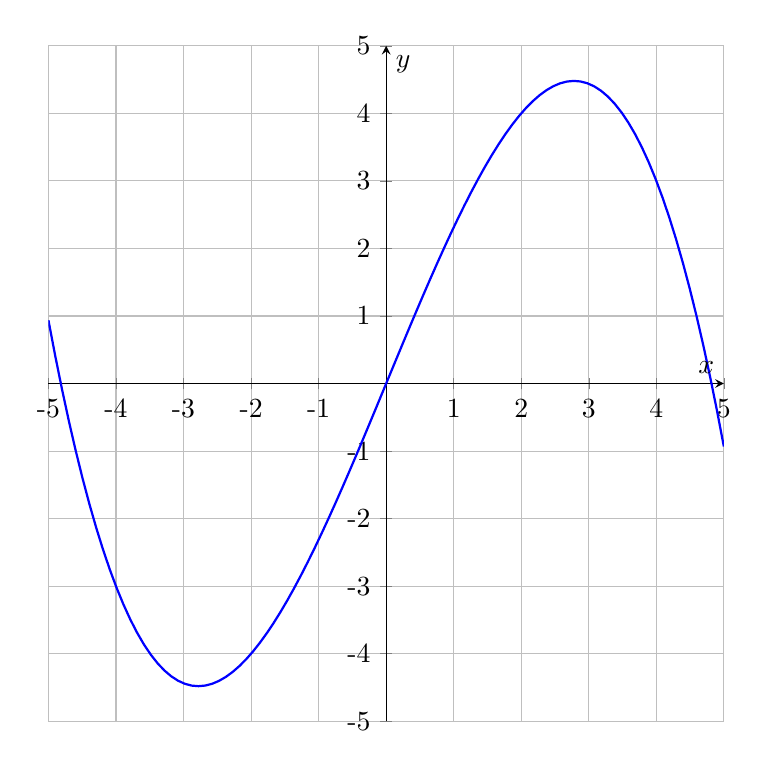
\begin{tikzpicture}
    \begin{axis}[
        axis lines = middle,
        xlabel = {$x$},
        ylabel = {$y$},
        xtick={-5,-4,-3,-2,-1,1,2,3,4,5},
        xticklabels={-5,-4,-3,-2,-1,1,2,3,4,5},
        ytick={-5,-4,-3,-2,-1,1,2,3,4,5},
        yticklabels={-5,-4,-3,-2,-1,1,2,3,4,5},
        xmin = -5, xmax = 5,
        ymin = -5, ymax = 5,
        grid = both,
        width = 4in,
        height = 4in,
        legend pos = north west,
    ]
    \addplot [
        domain=-5:5, 
        samples=100, 
        color=blue,
        thick,
    ]{-0.104167*x^3+2.41667*x};
    
    \end{axis}
\end{tikzpicture}

What is the remainder when $p(x)$ is divided by $x-4$?

\begin{choices} 
	\choice $-3$
	\choice $-2$
	\choice $2$
	\correctchoice $3$
\end{choices}

\vfill

%: Even graph
\question Describe the function.

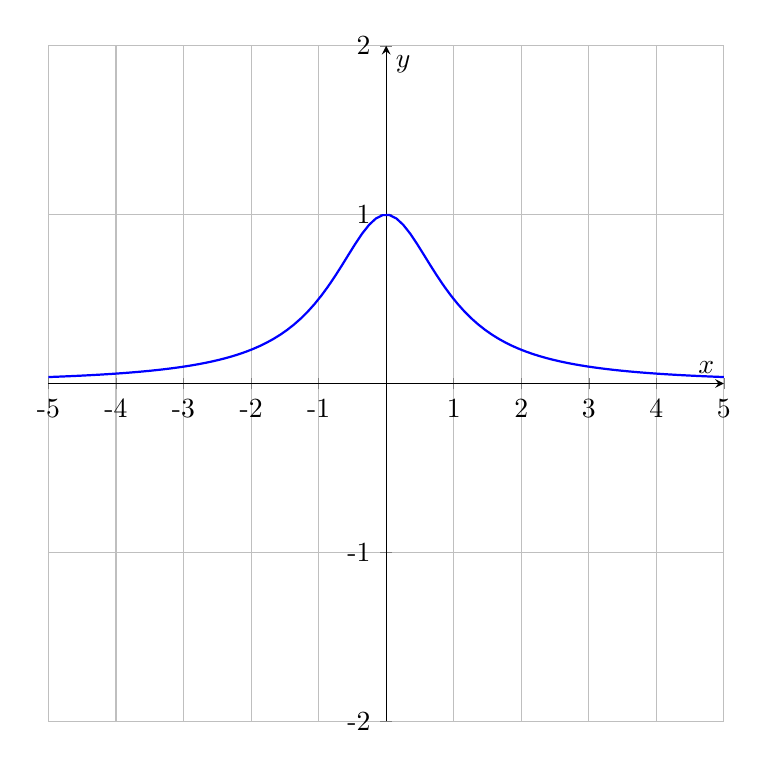
\begin{tikzpicture}
    \begin{axis}[
        axis lines = middle,
        xlabel = {$x$},
        ylabel = {$y$},
        xtick={-5,-4,-3,-2,-1,1,2,3,4,5},
        xticklabels={-5,-4,-3,-2,-1,1,2,3,4,5},
        ytick={-2,-1,1,2},
        yticklabels={-2,-1,1,2},
        xmin = -5, xmax = 5,
        ymin = -2, ymax = 2,
        grid = both,
        width = 4in,
        height = 4in,
        legend pos = north west,
    ]
    \addplot [
        domain=-5:5, 
        samples=100, 
        color=blue,
        thick,
    ]{1/(x^2+1)};
    
    \end{axis}
\end{tikzpicture}

The function is:

\begin{choices} 
	\choice odd.
	\correctchoice even.
	\choice one-to-one.
	\choice periodic.
\end{choices}

\vfill

\newpage

%: Odd graph
\question Describe the function.

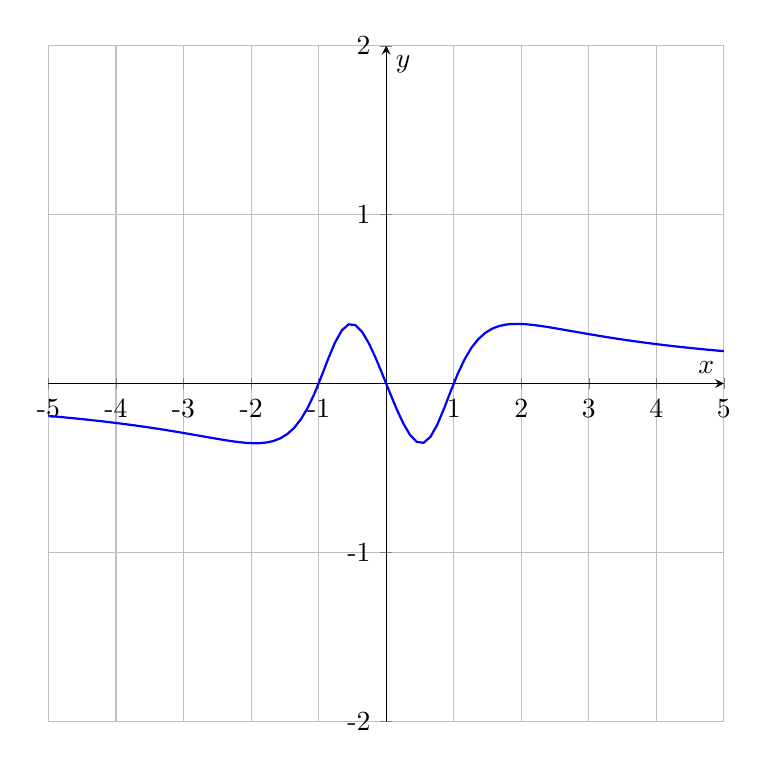
\begin{tikzpicture}
    \begin{axis}[
        axis lines = middle,
        xlabel = {$x$},
        ylabel = {$y$},
        xtick={-5,-4,-3,-2,-1,1,2,3,4,5},
        xticklabels={-5,-4,-3,-2,-1,1,2,3,4,5},
        ytick={-2,-1,1,2},
        yticklabels={-2,-1,1,2},
        xmin = -5, xmax = 5,
        ymin = -2, ymax = 2,
        grid = both,
        width = 4in,
        height = 4in,
        legend pos = north west,
    ]
    \addplot [
        domain=-5:5, 
        samples=100, 
        color=blue,
        thick,
    ]{(x^3-x)/(x^4+1)};
    
    \end{axis}
\end{tikzpicture}

The function is:

\begin{choices} 
	\correctchoice odd.
	\choice even.
	\choice one-to-one.
	\choice periodic.
\end{choices}

\vfill

%: One-to-one graph
\question Describe the function.

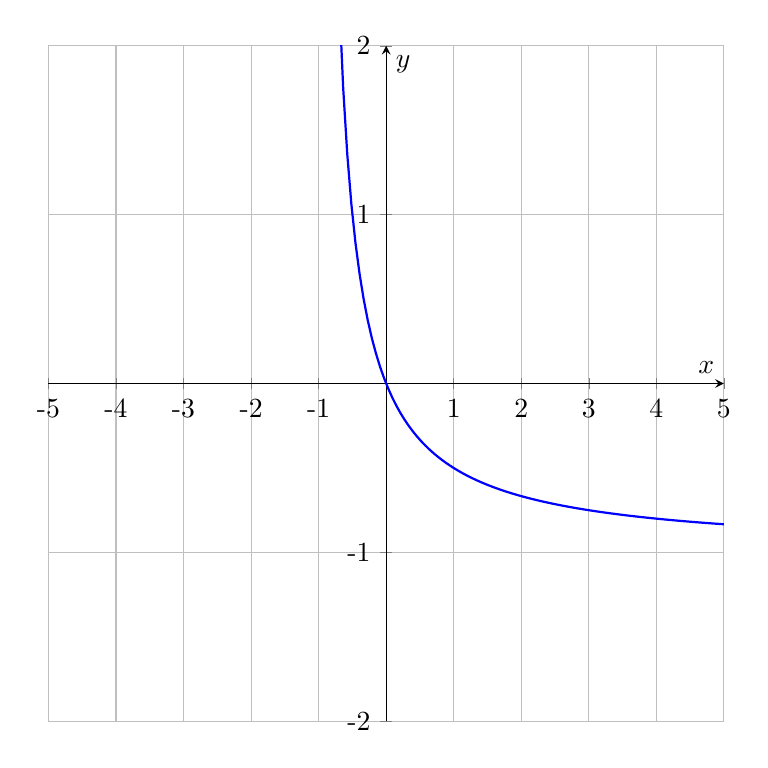
\begin{tikzpicture}
    \begin{axis}[
        axis lines = middle,
        xlabel = {$x$},
        ylabel = {$y$},
        xtick={-5,-4,-3,-2,-1,1,2,3,4,5},
        xticklabels={-5,-4,-3,-2,-1,1,2,3,4,5},
        ytick={-2,-1,1,2},
        yticklabels={-2,-1,1,2},
        xmin = -5, xmax = 5,
        ymin = -2, ymax = 2,
        grid = both,
        width = 4in,
        height = 4in,
        legend pos = north west,
    ]
    \addplot [
        domain=-1:5, 
        samples=100, 
        color=blue,
        thick,
    ]{1/(x+1)-1};
    
    \end{axis}
\end{tikzpicture}

The function is:

\begin{choices} 
	\choice odd.
	\choice even.
	\correctchoice one-to-one.
	\choice periodic.
\end{choices}

\vfill

\newpage


\ifStan{
%: cubic from rational roots
\question Which of the following cubic polynomial functions has roots at $\frac{3}{7}$ and $\frac{2}{5}$ and $-1$?

\begin{choices} 
	\correctchoice $y=35x^3+6x^2-23x+6$
	\choice $y=35x^3-6x^2-23x-6$
	\choice $y=6x^3+23x^2+6x-35$
	\choice $y=6x^3-23x^2+6x+35$
\end{choices}

\vfill

%: Find cubic with complex root and real root
\question Which polynomial function has roots of $-1$ and $3+2i$?

\begin{choices} 
	\choice $f(x)=x^3-5x^2-x+5$
	\correctchoice $f(x)=x^3-5x^2+7x+13$
	\choice $f(x)=x^3-7x^2+11x-5$
	\choice $f(x)=x^3-7x^2+19x-13$
\end{choices}

\vfill

% %: Profit
% \question A manufacturing company uses the following cost model:
% $$C(x)=0.18x^3+0.02x^2+4x+180$$
% where $x$ is the number of sprockets sold, in thousands. The sale price is modeled by another polynomial function:
% $$S(x)=95.4-6x$$
% And the company's revenue can be modeled as the product of the number of sprockets times the sale price of each sprocket.
% $$R(x)=x\cdot S(x)$$
% The profit is the difference of revenue minus cost.
% $$P(x)=R(x)-C(x)$$
% Find a polynomial expression for the profit function.
% 
% \begin{choices} 
% 	\choice $P(x)=0.18x^3+6.02x^2+91.4x+180$
% 	\choice $P(x)=0.18x^3-5.98x^2-91.4x+180$
% 	\correctchoice $P(x)=-0.18x^3-6.02x^2+91.4x-180$
% 	\choice $P(x)=0.18x^3+5.98x^2+99.4x+180$
% \end{choices}
% 
% \vfill


\newpage
}

All questions on this page refer to the function plotted below. Assume the domain of the function is from -5 to 5.

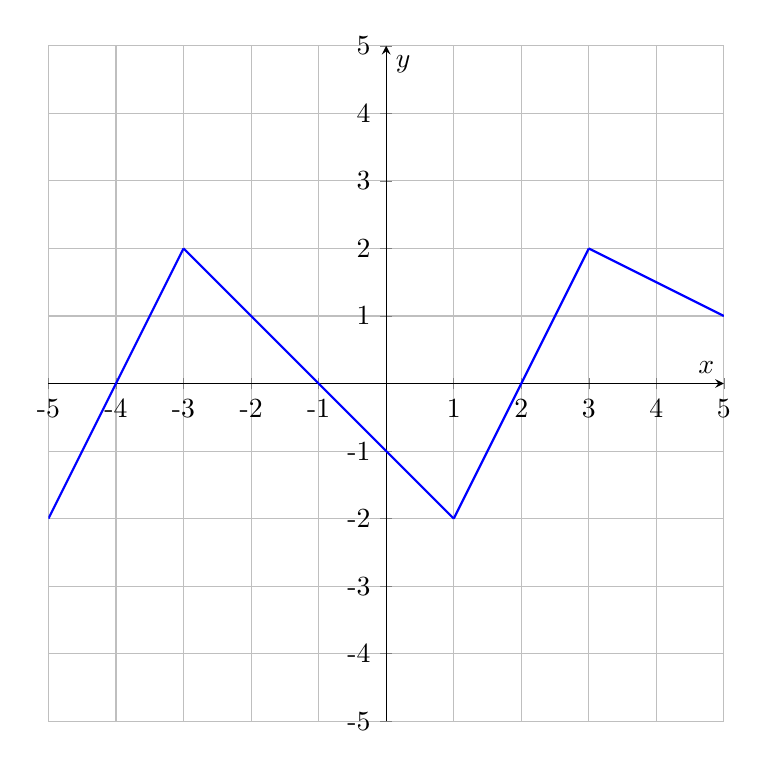
\begin{tikzpicture}
    \begin{axis}[
        axis lines = middle,
        xlabel = {$x$},
        ylabel = {$y$},
        xtick={-5,-4,-3,-2,-1,1,2,3,4,5},
        xticklabels={-5,-4,-3,-2,-1,1,2,3,4,5},
        ytick={-5,-4,-3,-2,-1,1,2,3,4,5},
        yticklabels={-5,-4,-3,-2,-1,1,2,3,4,5},
        xmin = -5, xmax = 5,
        ymin = -5, ymax = 5,
        grid = both,
        width = 4in,
        height = 4in,
    ]
    \addplot [
        domain=-5:-3, 
        samples=100, 
        color=blue,
        thick,
    ]{2*(x+5)-2};
    \addplot [
        domain=-3:1, 
        samples=100, 
        color=blue,
        thick,
    ]{-x-1};
    \addplot [
        domain=1:3, 
        samples=100, 
        color=blue,
        thick,
    ]{2*(x-1)-2};
    \addplot [
        domain=3:5, 
        samples=100, 
        color=blue,
        thick,
    ]{-1/2*(x-3)+2};
    
    \end{axis}
\end{tikzpicture}

%: interval of positivity
\question Over which of the following intervals is the function {\bf positive} for all values of $x$?

\begin{choices} 
	\correctchoice $(-4,-1) \cup (2,5)$
	\choice $(-5,-4) \cup (-1,2)$
	\choice $(-5,-3) \cup (1,3)$
	\choice $(-3,1) \cup (3,5)$
\end{choices}

\vfill

%: interval of decrease
\question Over which of the following intervals is the function {\bf decreasing} for all values of $x$?

\begin{choices} 
	\choice $(-4,-1) \cup (2,5)$
	\choice $(-5,-4) \cup (-1,2)$
	\choice $(-5,-3) \cup (1,3)$
	\correctchoice $(-3,1) \cup (3,5)$
\end{choices}

\vfill


\newpage

%: FR sketch factored polynomial
\question (10 points) Sketch the factored-form polynomial function on the {\bf Answer Sheet}. %the axes below.
$$y=-(x+3)^2(x-5)(x+7)(x-8)^2$$

% \vspace{1cm}
% 
% \begin{tikzpicture}
%     \begin{axis}[
%         axis lines = middle,
%         xlabel = {$x$},
%         ylabel = {$y$},
%         ytick=\empty,
%         yticklabels={},
%         xmin = -12, xmax = 12,
%         ymin = -5, ymax = 5,
%         % grid = both,
%         xtick={-10,-9,-8,-7,-6,-5,-4,-3,-2,-1,1,2,3,4,5,6,7,8,9,10},
%         width = 6in,
%     ]
%     \end{axis}
% \end{tikzpicture}

\vfill

% %: FR factor cubic (x+1)(x-2)(x+3)=x^3+2x^2-5x-6
% \question Express $x^3+2x^2-5x-6$ in factored form. Please box your final answer.
% 
% \vfill


\end{questions}

\end{document}
